\chapter{Introducción}

En una era digital donde las tendencias cambian en un abrir y cerrar de ojos, los memes se han convertido en una forma popular de comunicación que se mantiene atemporal y relevante cambiando y adaptándose por cada tendencia.

Los memes están tan integrados en nuestra cultura que los utiliza desde el estudiante que busca hacer sus presentaciones y exposiciones más memorables y llevaderas hasta una empresa que busca captar la atención de audiencia en las redes sociales.

La integración de los memes en el contenido no solo buscan vender el contenido de manera más fresca, entretenida y atractiva, sino que otras veces, solo se busca el entretenimiento y la diversión pura y simple de los consumidores.

Imagine una escena en la que un grupo de amigos se reúne y discuten sobre los últimos acontecimientos políticos cuando, de repente, un meme ingenioso y fuera de lugar se convierte en el centro de la conversación, rompiendo el hielo y generando risas. Imagine ahora una situación, en un entorno académico, en el que un estudiante quiere realizar una presentación algo diferente y para ello decide introducir algún meme. Esta situación no únicamente se da en un entorno académico, sino que incluso en charlas llevadas por ponentes profesionales. Cada vez es más común encontrar algún meme que otro con el fin de que estas charlas sean más `digeribles`. Un claro ejemplo de este caso es Miguel Ángel Durán (\href{https://midu.dev/}{@midudev}), un experto en desarrollo de software, actualmente divulgador sobre programación, estrella de GitHub y Microsoft MVP, el cual es conocido por su habilidad para integrar memes de forma creativa y efectiva en sus charlas y presentaciones.

\begin{figure}[ht]
    \caption{Pierde el miedo a desplegar a producción en viernes de \href{https://midu.dev/}{Miguel Ángel Durán} y \href{https://platzi.com/}{Platzi}en \href{https://platzi.com/conf/}{Platzi Conf} \cite{confe}.}
    \centering
    \vspace*{0.5cm}
    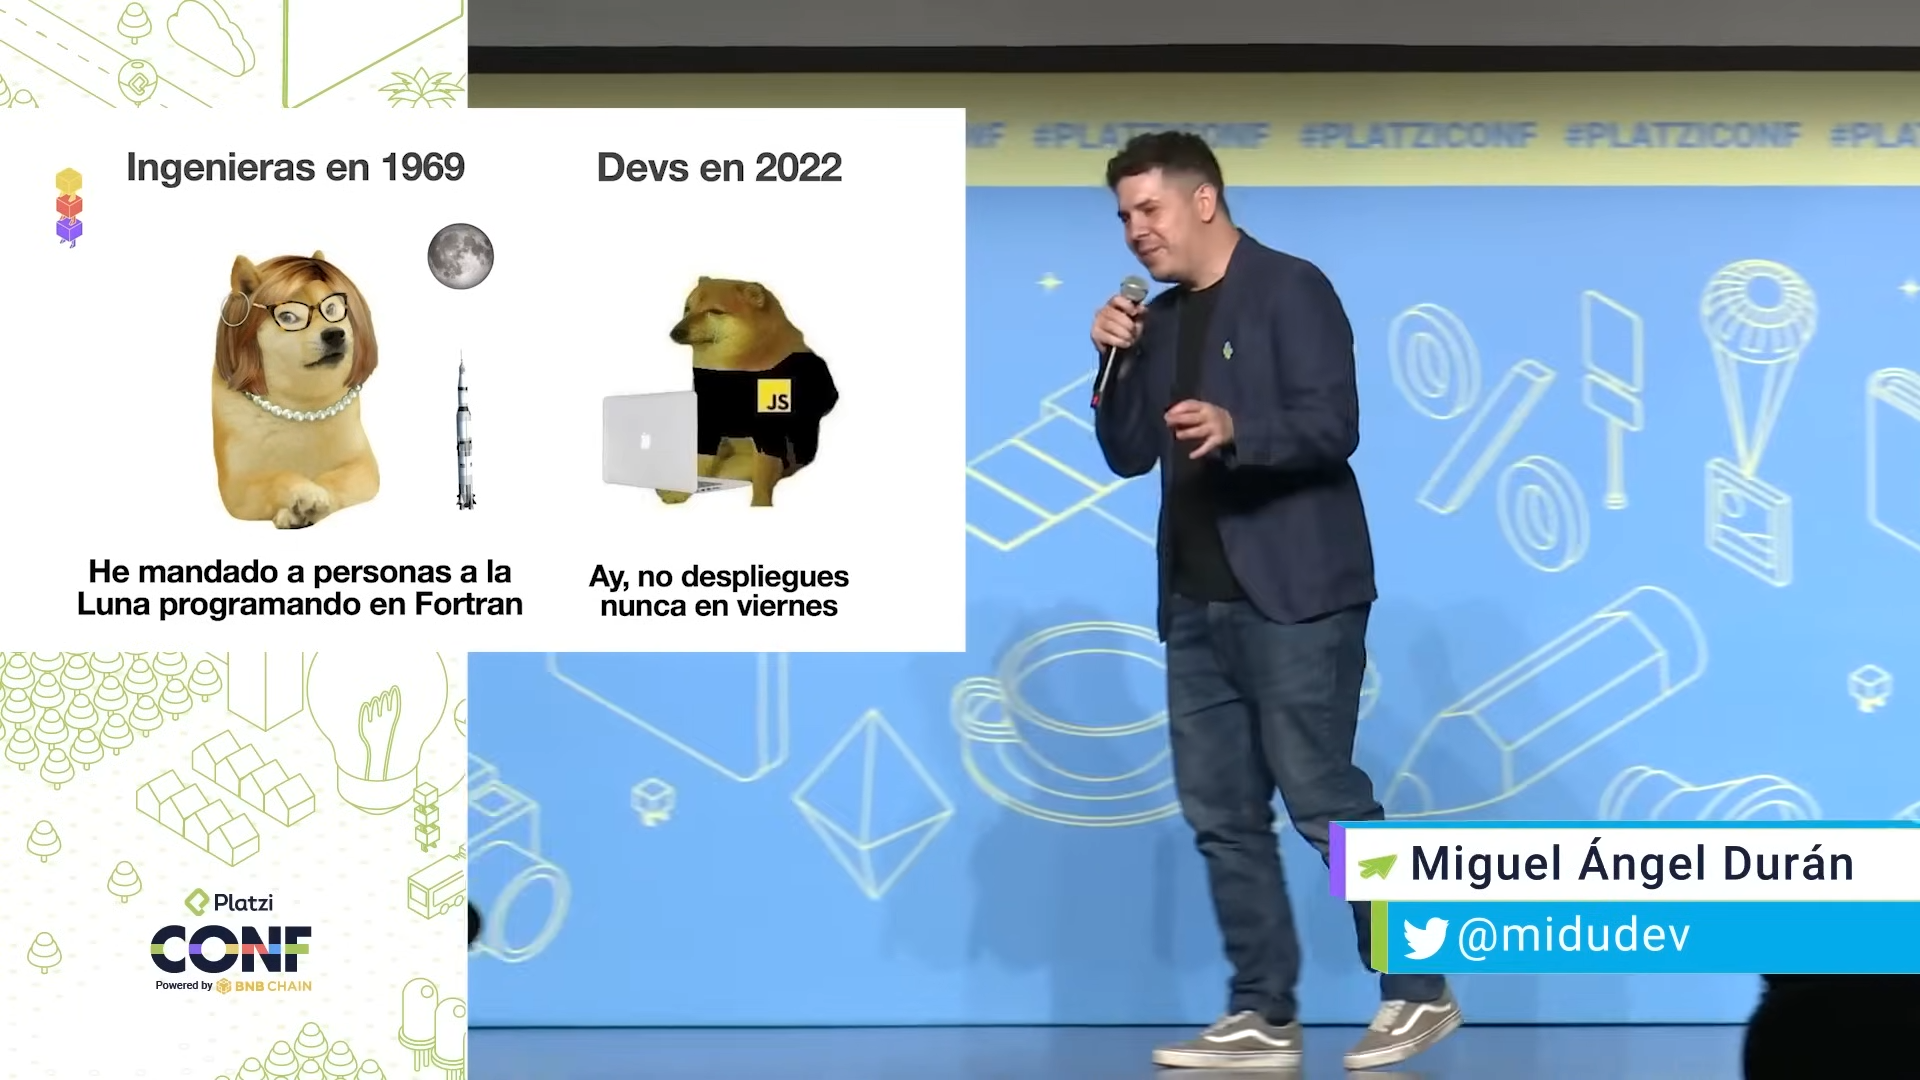
\includegraphics[scale=0.15]{figuras/platziconfmidudev.png}
\end{figure}

En todos estos casos y en muchos más, los memes se han convertido un medio para conectar con el consumidor de una manera única y efectiva.

Sin embargo, a pesar de su uso generalizado, la gestión, centralización y organización de memes sigue siendo un desafío para muchos creadores de contenido, empresas y personas.

\section{Motivación}

Como hemos comentado la creación y compartición de memes es una actividad de lo más habitual por lo que la falta de un sistema centralizado limita su potencial para todo tipo de usuarios. Esta falta de una solución informática específica se traduce en una pérdida de tiempo y recursos, así como en una limitación en la capacidad de generar contenido relevante y oportuno. Lo cual es una característica esencial en el mundo de los memes.

La motivación detrás de este proyecto radica en ofrecer una solución que subsane las dificultades que los usuarios encuentran a la hora de gestionar estos medios de información. Estas dificultades van desde la dificultad de encontrar memes antiguos hasta la falta de herramientas colaborativas y centralizadas. Como se puede apreciar los problemas pueden llegar a ser muy diversos y afectar a diferentes tipos de usuarios.

El proyecto `Memes para todos` aspira a proporcionar una plataforma robusta y fácil de usar que simplifique el proceso de creación, almacenamiento y distribución de memes para todo tipo de usuarios, sin importar su experiencia previa o contexto.

\section{Definición del problema}

Dentro de este marco de trabajo, para realizar una mejor de definición del problema, se han identificado una serie de personas con necesidades y objetivos específicos que junto con las historias de usuario describen los problemas que se pretenden resolver con este proyecto.

La identificación de los usuarios es un paso fundamental para el desarrollo del proyecto, ya que permite definir mejor las necesidades, requisitos, deseos, expectativas del usuario final que hará empleo de la solución. Además, estos usuarios sirven para la validación de la solución propuesta.

La metodología utilizada ha sido la de `personas`. Esta técnica se basa en la representación ficticia, pero concreta del grupo de usuarios al que va dirigido nuestra solución. El fin de este análisis es el poder llevar a cabo una compresión clara de los objetivos y necesidades de los usuarios en contextos específicos de uso.

\subsection{Usuarios identificados}

    \subsubsection{Cristina Contreras Márquez (estudiante de ingeniería informática)}

    Cristina Contreras Márquez es una estudiante de ingeniería informática que, como cualquier otro estudiante, necesita hacer presentaciones para exponer sus trabajos. Cristina es una persona creativa que siempre le gusta aportar su esencia a las presentaciones las cuales vuelve únicas y diferentes. Cristina siempre está buscando encontrar una forma fácil y rápida de hacer esos memes que se le van ocurriendo mientras elabora la presentación.

    \subsubsection{Ted Johnson González (experto conferenciante)}

    Ted Johnson González es un experto en oratoria que realiza muchas ponencias y charlas. Ted es un ponente profesional que siempre busca la manera de hacer sus charlas más amenas y entretenidas. La característica diferenciadora e innovadora de sus conferencias es la inclusión de memes que ayudan a reforzar su discurso y aumentar la retención del contenido por parte de la audiencia gracias a la conexión con el meme.

    \subsubsection{Departamento de marketing de Corporate Solutions}

    El departamento de marketing de `Corporate Solutions` le ha expresado al CTO en la empresa, la necesidad de un sistema centralizado para agilizar el proceso de generación y gestión de multimedia (principalmente memes). La adopción de una solución de este tipo permitiría a los miembros del equipo de marketing colaborar de manera más eficiente y efectiva, así como garantizar la coherencia y calidad del contenido generado.

\section{Historias de usuario}

    \subsection{Cristina Contreras Márquez (estudiante de ingeniería informática)}

        \begin{enumerate}
            \item [HU01] Como Cristina Contreras Márquez, estudiante de Ingeniería Informática, desearía un sistema donde poder ir confeccionando memes a partir de plantillas (para hacerlos más rápido) a medida que se me van ocurriendo mientras elaboro la presentación.
            \item [HU02] Como Cristina Contreras Márquez, estudiante de Ingeniería Informática, me gustaría poder elegir entre una serie de memes predefinidos o hechos por mí para poder añadirlos a mis presentaciones.
        \end{enumerate}

    \subsection{Ted Johnson González (experto conferenciante)}

        \begin{enumerate}
            \item [HU03] Como Ted Johnson González, experto conferenciante, necesito un sistema que me permita encontrar memes relevantes y atractivos para incluir en mis presentaciones.
            \item [HU04] Como Ted Johnson González, experto conferenciante, necesito una herramienta que me permita personalizar y adaptar los memes a mi estilo y contenido.
        \end{enumerate}

    \subsection{Departamento de marketing de Corporate Solutions}

        \begin{enumerate}
            \item [HU05] Como departamento de marketing, nos gustaría tener un sistema centralizado que nos permita de forma centralizada generar y gestionar multimedia.
            \item [HU06] Como departamento de marketing, necesitaríamos una herramienta que nos permita colaborar en un meme varios miembros del equipo.
        \end{enumerate}

\section{Objetivos Iniciales}

\begin{enumerate}
    \item Diseñar una solución que sea lo más económica posible, permitiendo su instalación en servidores en la oficina o su despliegue en contenedores sin costos excesivos, lo que garantiza una mayor accesibilidad y viabilidad para organizaciones de todos los tamaños y presupuestos.
    \item Se deberá crear un sistema que comprenda una gama de clientes lo más amplia posible, ofreciendo una solución que sea capaz de adaptarse a las diferentes necesidades y preferencias de los usuarios.
    \item Se deberá garantizar la accesibilidad y facilidad de uso desarrollando una aplicación que se pueda utilizar incluso desde un ordenador de bajas prestaciones.
    \item La licencia del proyecto deberá de permitir su uso por cualquier organización o personas sin importar el fin con el que se utilice, ya sea para uso personal, educativo o empresarial.
\end{enumerate}